\textcolor{orange}{\chapter{De la bible au Big Bang!}}
\section{Hypothèse du big bang}
\paragraph{}
	\begin{wrapfigure}[14]{l}{155px}
	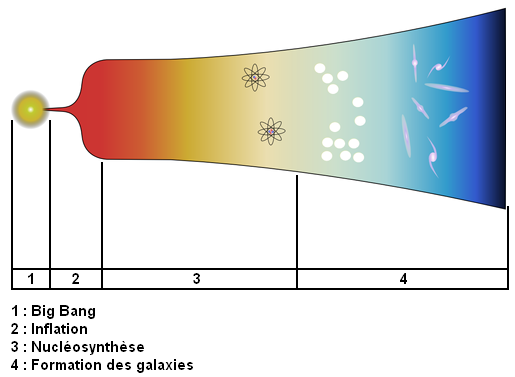
\includegraphics[width=150px]{img3.png}
	\caption{Hypothèse du Big Bang}
\end{wrapfigure}
Comme tout le monde le sait, il existe plusieurs hypothèses sur le sujet, 
et aucune n'est sûr encore de nos jours ce sont des théories. \\
La naissance de l'Univers est sans aucun doute le grand débat cosmologique de ce 
siècle. Deux grandes théories se sont affrontés. Finalement, l'une l'a emporté 
sur l'autre, mais comment les scientifiques ont-ils pu affirmer que l'une était 
correcte contrairement à l'autre ?\\
Ces deux grandes théories ont essayé d'expliquer l'origine de l'Univers. 
La première, la théorie du \textbf{\textsc{Big Bang}}, affirme que l'Univers à 
commencé par une explosion massive en un seul point de l'espace il y a environ 
quinze milliards d'années.\\ \\ \\ \\ \\

Les anciennes religions polythéistes qu'en à elles se rapprochent étrangement de
du Big Bang car tout naitrait du Chaos, celui ci donna naissance à la Terre
\footnote{Représenté par la Déesse Gaia}, qui créa le Ciel, le Temps
\footnote{Représenté par Chronos} ainsi que la Vie et la Mort
\footnote{Représenté par Rhéa et les Titans}, ces derniers procréèrent les 
autres dieux qui représente toutes choses existant dans notre monde et utile 
à l'Univers.

\begin{figure}[h]
	\begin{center}
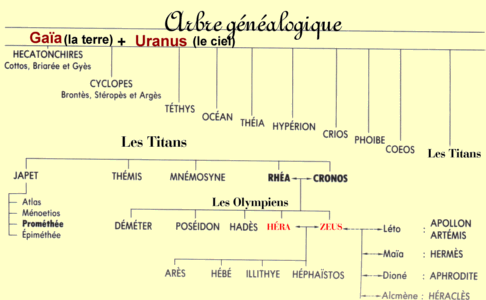
\includegraphics[width=200px]{img4.png}
\caption{Descendance de Gaia}
	\end{center}
\end{figure}

\section{Hypothèse de la création continue}
\paragraph{}
D'après la deuxième théorie, celle de la création continue, il n'y aurait pas eu
de Big Bang. L'univers à toujours existé et existera toujours. Elle envisage un
univers dans lequel les vieilles galaxies ont continuellement disparu au-delà de
l'horizon cosmologique pour être remplacée par de nouvelles galaxies faites de
matière issue du néant. Pour les scientifiques, ces deux théories sont 
invraisemblables, les scientifiques s'intéressant essentiellement 
aux preuves.\\
				  
Si la théorie de la création continue est exacte, l'Univers aurait dû présenter
il y a des millions d'années le même visage qu'aujourd'hui. Or les astronomes 
ont découvert que ce n'était pas le cas, autrefois, les galaxies étaient 
réparties différemment dans l'espace et il y avait plus de quasars
\footnote{Source de rayonnement quasi-stellaire, galaxie lointaine}. 
La théorie de la création continue semble donc inexacte. \\
	   
\section{Hypothèse religieuse}
Cependant cette deuxième théorie peut se raccrocher à une autre vision de la 
naissance du monde dans la religion cette fois ci dites Moderne.\\
Dans une religion, la création apporte une explication du commencement du monde. 
Le monde serait créé par une ou plusieurs divinités. Ces explications ne sont 
pas justifiées, elles sont <<révélées>> autrement dit, les religions demandent 
d'y croire. \\
		
Dans les religions du livre (judaïsme, christianisme et islam), 
 la création est décrite par des chapitres ou des versets des livres saints. \\
Dans la religion hébraïque, la création est décrite dans le livre de la Genèse, 
 qui est le premier livre de la Torah. Dieu aurait créé le monde et la vie en 
 six jours, et se serait reposé le septième. Le récit de la création est 
 similaire dans la religion chrétienne.

\begin{itemize}
\item \textbf{Premier jour:} Création de la terre, puis de la lumière, du jour 
	et de la nuit. \\
\item \textbf{Deuxième jour:} Création du firmament et du ciel. \\
\item \textbf{Troisième jour:} Séparation de l'eau du sec et création de la mer 
	et des continents. Création de la nature, des arbres et des fruits. \\
\item \textbf{Quatrième jour:} Création des étoiles et des saisons. \\
\item \textbf{Cinquième jour:} Création des poissons et des oiseaux, et de la 
	procréation des animaux. \\
\item \textbf{Sixième jour:} Création des animaux domestiques, des reptiles et 
	des serpents. Création du jardin d Éden, du premier homme Adam à son image
	à partir de la poussière, et de la première femme à partir de la côte de 
	l'homme. \\
\item \textbf{Septième jour:} Repos \\
\end{itemize}

Cependant aucun écrit sur l'Univers ni de ce qu'il pouvait exister avant la 
création du monde, c'est pour cela que cette théorie et de plus en plus 
obsolètes de nos jours.

	\begin{figure}[h]
		\begin{center}
	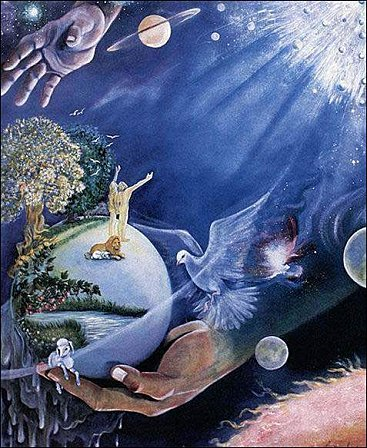
\includegraphics[width=100px]{img5.png}
	\caption{Créationnisme}
		\end{center}
	\end{figure}
	
\textcolor{orange}{\chapter{Confrontation entre la Science et la Religion : 
		Des freins au progrès scientifique ?}}

Avant de commencer... \\
Des préalables pour calmer le débat...\\ 

\paragraph{Les croyants ne sont pas tous créationnistes...}Croire en un Dieu est 
tout à fait compatible avec l'étude des sciences. On peut avoir des croyances et
aussi comprendre le monde qui nous entoure. Le créationniste à une lecture 
littérale des textes religieux, alors que le croyant sait qu'il faut interpréter
les textes.

\paragraph{Les évolutionnistes ne sont pas tous athées...} Cela n'a rien à voir.
L'étude de la nature, de la faune, de l'astronomie et des mécanismes qui les 
régissent n'empêche pas de croire en un Dieu pour, par exemple, donner un sens à
sa vie.

\paragraph{}Croire et comprendre, ou Croire ou comprendre... tel est la 
	question !  \\
Depuis des siècles ce débat fait rage entre la science et la religion notamment
pour l'age du Monde et de l'Univers, les premiers à avoir aborder le sujet étant 
la religio...

\paragraph{Saint Augustin}Admet la date d'environ 5000 ans av. J.-C. pour la 
création de l'Univers\footnote{date donnée à partir de la Genèse}\\
Dernière glaciation, et départ de notre civilisation: environ 10 000 ans av. 
J.-C.

\paragraph{Aristote}Comme la plupart des philosophes grecs, il n'aimait pas 
l'idée de création car elle présentait un arrière-goût d'intervention divine.
\\ Il croyait par conséquent que la race humaine et le monde qui l'entoure 
existaient et existeraient à jamais.

\paragraph{Ussher}
L'archevêque irlandais James Ussher avait déterminé que le monde commençât en
4004 av. J.-C., d'après les Saintes Écritures. 

\begin{itemize}
\item Il étudie la chronologie des patriarches, des juges, des prêtres et des 
	rois. 
\item Il commence par Adam qui est réputé avoir vécu 930 ans et suit les 
	générations. 
\end{itemize}

Publiées en 1650 dans les annales de l'Ancien et du Nouveau Testament, 
les conclusions de Ussher sont très vite acceptées comme définitives par
le clergé.

\paragraph{Buffon}
C'est seulement 150 ans plus tard que Buffon suggère que la Terre pourrait 
avoir 75 000 ans. \\
Il est durement critiqué par l'eglise et doit sous l'autorité du clergé revoir 
ces calculs à la baisse car ils ne correspondent pas au écrit, ce qui emmene 
donc à dire que la religion avait l'autorité sur le savoir et les sciences,
 ce qui laisse à penser que rien n'est exact à cette époque

\paragraph{}
Il faudra encore 50 ans pour que la lecture des couches géologiques renvoie au 
musée les mathématiques généalogiques et théologiques de l'archevêque anglican 
d'Armagh\\
Ce n'est qu au $XX^{éme}$ siécle que les scientiques ne dépendant plus de l'autorité
religieuse commencérent à affirmer que l'Univers daté d'approximativement de 
quinze milliards d'années ce qui ne laissa pas l'Eglise indiferrente, mais
cette fois si impuissante .

	\begin{figure}[h]
		\begin{center}
	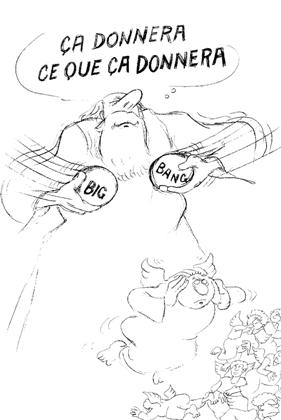
\includegraphics[width=250px]{img6.png}
	\caption{Et Dieu Créa le Big Bang}
		\end{center}
	\end{figure}

